\chapter{Klasifikace pózy}
\label{sec:PoseClassification}

Problematika vyhodnocování je velmi široká a přináší mnoho problémů. Ostatně i
člověk někdy může špatně interpretovat chování druhé osoby. Například pokud
někdo skáče do postele či jinak prudce lehá, může to vypadat jako nebezpečná
situace. Stejně se v počítačovém vidění nevyhneme falešným poplachům, nicméně
se budeme snažit zapojit různě techniky pro zlepšení přesnosti našeho
detektoru.

Cílem této části práce je vytvořit algoritmus, který pro danou pózu
(reprezentovanou klíčovými body), resp. sekvenci takových póz (získané pro
jednu osobu ze sekvence snímků), určí, zda se jedná o situaci pádu, či nikoliv.
Tento algoritmus bude přijímat vždy pózu jedné osoby, funkcionalita pro více
osob bude řešená v další části práce.

\section{Trénovací data}

Pro trénování našeho modelu jsme použili více než 150 videi. Pro videa byly
vytvořeny anotace aktuální třídy pózy. Tato anotace není pro každý snímek, ale
pouze při změně definuje časovou značku a následující třídu.

Dále byl vytvořen skript, který prošel každé video a vytvořil trénovací data
pro další fázi. Ty obsahují pro každý snímek detekované klíčové body (jako
vstup) a aktuální třídu (jako požadovaný výstup). Pro detekci byl použit dříve
vybraný algoritmus pro detekci pózy. Na použitém algoritmu by teoreticky
nemuselo záležet (pokud detekuje stejné typy klíčových bodů), je ale lepší
použít stejný algoritmus jak pro trénovací data, tak ve výsledném programu.
Algoritmy se totiž můžou v některých situacích chovat trochu jinak (např.
okluze) a náš model by tak dostával v praxi jiná data, než pro jaké byl
natrénován.

Pro trénovací data jsme použili 3 třídy, ty odpovídají třem různým třídám pózy,
které nás zajímají - \textit{normální}, kdy osoba např. chodí, sedí nebo stojí,
\textit{padá} - přechodný stav padání, definován od započatí pohybu směrem
dolů, a \textit{upadl} - definován od momentu, kdy se dotkl zemi trupem nebo
všemi končetinami.

Pro náš model obecně potřebujeme jenom dvě třídy - \textit{normální} a
\textit{upadl}. Nicméně budeme pro náš model experimentovat i s třetí třídou -
\textit{padá}, která pomůže síti hlouběji pochopit problematiku a přesněji
rozeznat některé situace, zejména pak v případě využití rekurentních
neuronových sítí.

\section{Dopředná neuronová síť}
Nejjednodušší architekturou, kterou můžeme pro náš model použít, je dopředná
neuronová síť. Tento model pak bude klasifikovat jednotlivé pózy, aniž by znal
jejich kontext. Síť bude klasifikovat klíčové body pouze podle aktuální
lokalizace ve snímku, nikoliv podle pohybu.

Výhodou této architektury je jednoduchost, potažmo rychlost. Síť nepotřebuje
mnoho parametrů a oproti rekurentním sítím, potřebuje pro evaluaci pouze jeden
dopředný průchod vrstvami sítě.

Další výhodou je jednoduchost trénování a používání. V případě více osob pro
samotnou klasifikaci pádu není nutné sledování osob. Můžeme jednoduše
klasifikovat všechny detekované pózy, aniž bychom řešili, které osobě patří.

Tato síť ale ve výsledku bude klasifikovat pózy pouze dle vzájemného umístění
jednotlivých klíčových bodů, potažmo délky končetin, nebude ale brát v úvahu
natočení postavy. To proto, že postavy ve snímku vystupují pod různým úhlem
natočení v závislosti na natočení kamery. Naopak síť, která je schopná sledovat
pohyb, bude schopna sledovat mj. i změnu natočení postavy a to bez ohledu na
natočení kamery.

\section{Rekurentní neuronové sítě}

Rekurentní neuronové sítě (ang. Recurrent Neural Networks - RNN) je kategorie
neuronových sítí, které do své architektury zapojují zpětnou vazbu. Na rozdíl
od dopředných sítí, které spracovávájí jednotlivé vstupy nezávisle, rekurentní
sítě spolu s aktuálním vstupem při evaluaci zohledňují nějakým způsobem i
výsledek předchozí iterace. Jejich využití tedy je ve dvou oblastech: analýza
změn pozorovaného objektu v čase (např. sledování pohybu, analýza chování či
predikce časových řad) a zpracování kontextuálních informací jako je např.
přirozený jazyk.

Data, která v aktuální iteraci přebíráme z předchozí iterace, se často označují
jako skrytý stav (ang. hidden state). Je to forma paměti, která se s každou
iterací aktualizuje. Často je reprezentován jako stavová vrstva (ang. state
layer nebo context layer), která přijímá hodnoty z výstupu neuronů, uchovává je
mezi iteracemi a předává je spolu se vstupními daty na vstup neuronů. Na
obrázku \ref{fig:rnn} je tato vrstva reprezentována neurony $c_i$.

\begin{figure}[]
    \centering
    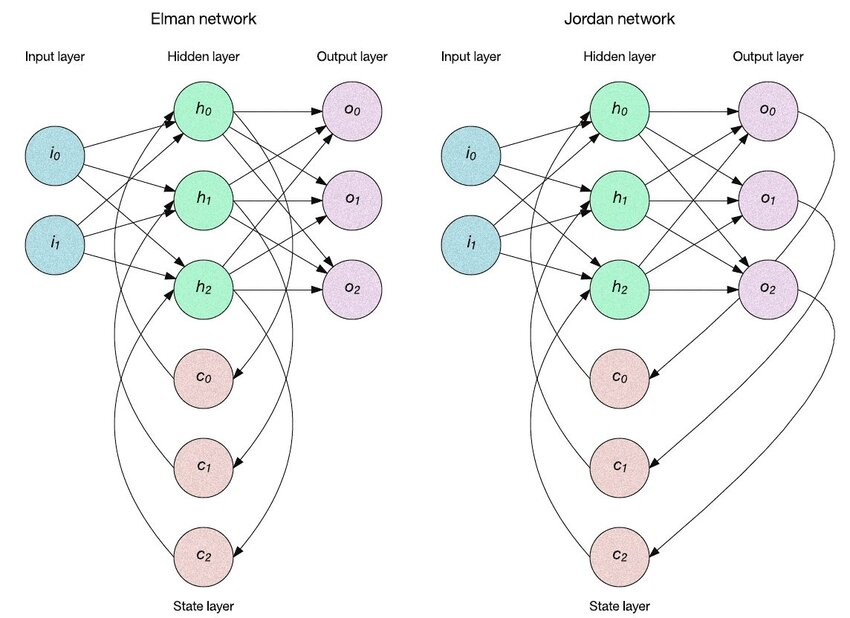
\includegraphics[width=0.8\textwidth]{Figures/rnn.png}
    \caption{Základní architektury RNN \cite{aksoy}}
    \label{fig:rnn}
\end{figure}

Nejjednodušší forma rekurentní neuronové sítě je NN s jednou skrytou vrstvou;
tato vrstva kromě dat ze vstupní vrstvy, přijímá také výstup předchozí iterace
buď svých vlastních neuronů, anebo z neuronů výstupní vrstvy, viz obrázek
\ref{fig:rnn}. Obrázek je zjednodušený, v praxi jsou stavová a skrytá vrstva
plně propojeny. Taky Tyto architektury se jmenují Elmanova síť \cite{elman},
resp. Jordanova síť \cite{jordan}, od jejích tvůrců. Tyto sítě jsou taky známé
jako jednoduché rekurentní sítě (ang. Simple Recurrent Networks - SRN). I když
pojem rekurentních sítí byl známy už od začátků neuronových sítí jako takových
a byly i případy jejích použití, právě tyto sítě patřily k prvním, které
používaly pro trénování algoritmus backpropagation. Jednoduché rekurentní sítě
uchovávají pouze krátkodobé vzory a jsou vhodné spíše pro jednoduché úlohy,
jako je např. predikce časových řad.

Stejně jako u dopředných neuronových sítí, kde se od jednoduchého perceptronu
přešlo k hlubokým sítím, se i rekurentní sítě rozšířily na více vrstev. V
hlubokých rekurentních neuronových sítích (ang. deep RNN - DRNN) jsou pak
jednotlivé vrstvy většinou podobné struktuře Elmanovy sítě - zpětná vazba je
předávána pouze v rámci jedné vrstvy, nikoliv mezi vrstvami RNN (například z
výstupní vrstvy do první skryté vrstvy). Má to několik důvodů. Trénování sítě
ze zpětnou vazbou mezi vrstvami by bylo velmi složité a obtížné. Taky, obecně
každá vrstva sítě se učí pochopit problém na jiné úrovní abstrakce, zpětná
vazba přes několik vrstev by pak mohla narušit stabilitu tohoto procesu a
omezit kvalitu učení.

Pro pochopení rekurentních neuronových sítí je třeba si vysvětlit, jak se
trénují. Pro vizualizaci trénování RNN se tyto sítě takzvaně rozbaluje v čase
(ang. unrolling). Znamená to, že jednotlivé iterace vizualizujeme jako sekvenci
stejných sítí (stejné váhy), které v čase $t$ přijímají vstup $x_t$ a vracejí
výstup $y_t$, viz obrázek \ref{fig:bptt}. Zároveň místo smyček znázorňujících zpětnou vazbu, přijímá skrytá
vrstva v čase $t$ stav $c_{t-1}$ z předchozí iterace. Takto je propojená mezi
iteracemi každá skrytá vrstva (na obrázku \ref{fig:bptt} vizualizováno propojení přes
stavovou vrstvu)

\begin{figure}[]
    \centering
    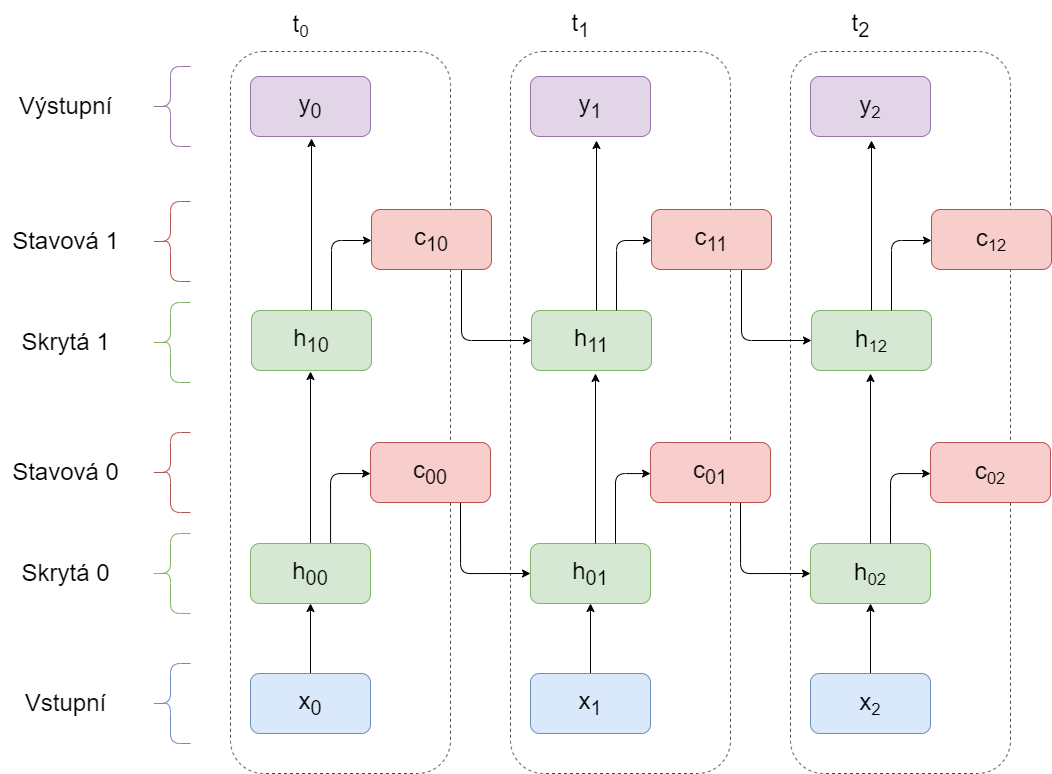
\includegraphics[width=0.7\textwidth]{Figures/BPTT_deep.png}
    \caption{Unrolling hluboké RNN}
    \label{fig:bptt}
\end{figure}

Při trénování se pak používá algoritmus zpětného šíření chyby v čase (ang.
backpropagation through time - BPTT). Algoritmus funguje stejně jako klasický
backpropagation, šíří se ale nejenom vrstvami ale i iteracemi. Unrolling nám
pomáhá backpropagation pochopit, jednotlivé iterace totiž jsou naskládáne jako
vrstvy.

Výše popsané základní rekurentní neuronové sítě, někdy označovány jako vanilla RNN, 


\endinput